\newChapter{Introduction}
\label{cha:introduction}

The Internet of Things \gls{IoT} is one of the most prolific domains in computer science
nowadays. There is connected object everywhere and the amount of data that we
receive from them is growing day after day. Everybody wants to measure some
environment variable using a simple and cheap device like an Arduino or a
Raspberry Pi.

In another hand, the people who want to use those devices are often not familiar
with the hardware and/or the software parts of an IoT project. For example, a
chemistry engineer could be interested to measure some value in the air, but he
is absolutely not in the IoT domain.

\section{Context}
\label{sec:intro-context}

Imagine an electrical engineer who needs to create a system which is able to
recover data from multiple sensors, like external temperature and barometric
pressure. With that data, the engineer need to compute a new pressure value
with the temperature and compare it to the one give by the barometric pressure
sensor using graph plot.

The problem for this electrical engineer is the software part. He doesn’t know how
to send data through the network, recover them and store them into a database
for a future plot. In another hand, if it’s a software engineer to do this, he
would not know the hardware part.

IoT programming is at some point a merge of some specific domain like Software,
Hardware, Telecommunication and Design. The figures \ref{fig:basic_archi} illustrate
this concept of multi-domain project. Are involve in this concept:

\begin{itemize}
\item Hardware
\item Software
\item Design
\item Telecommunication
\end{itemize}

\begin{figure}[ht]
  \centering
  \fbox{
    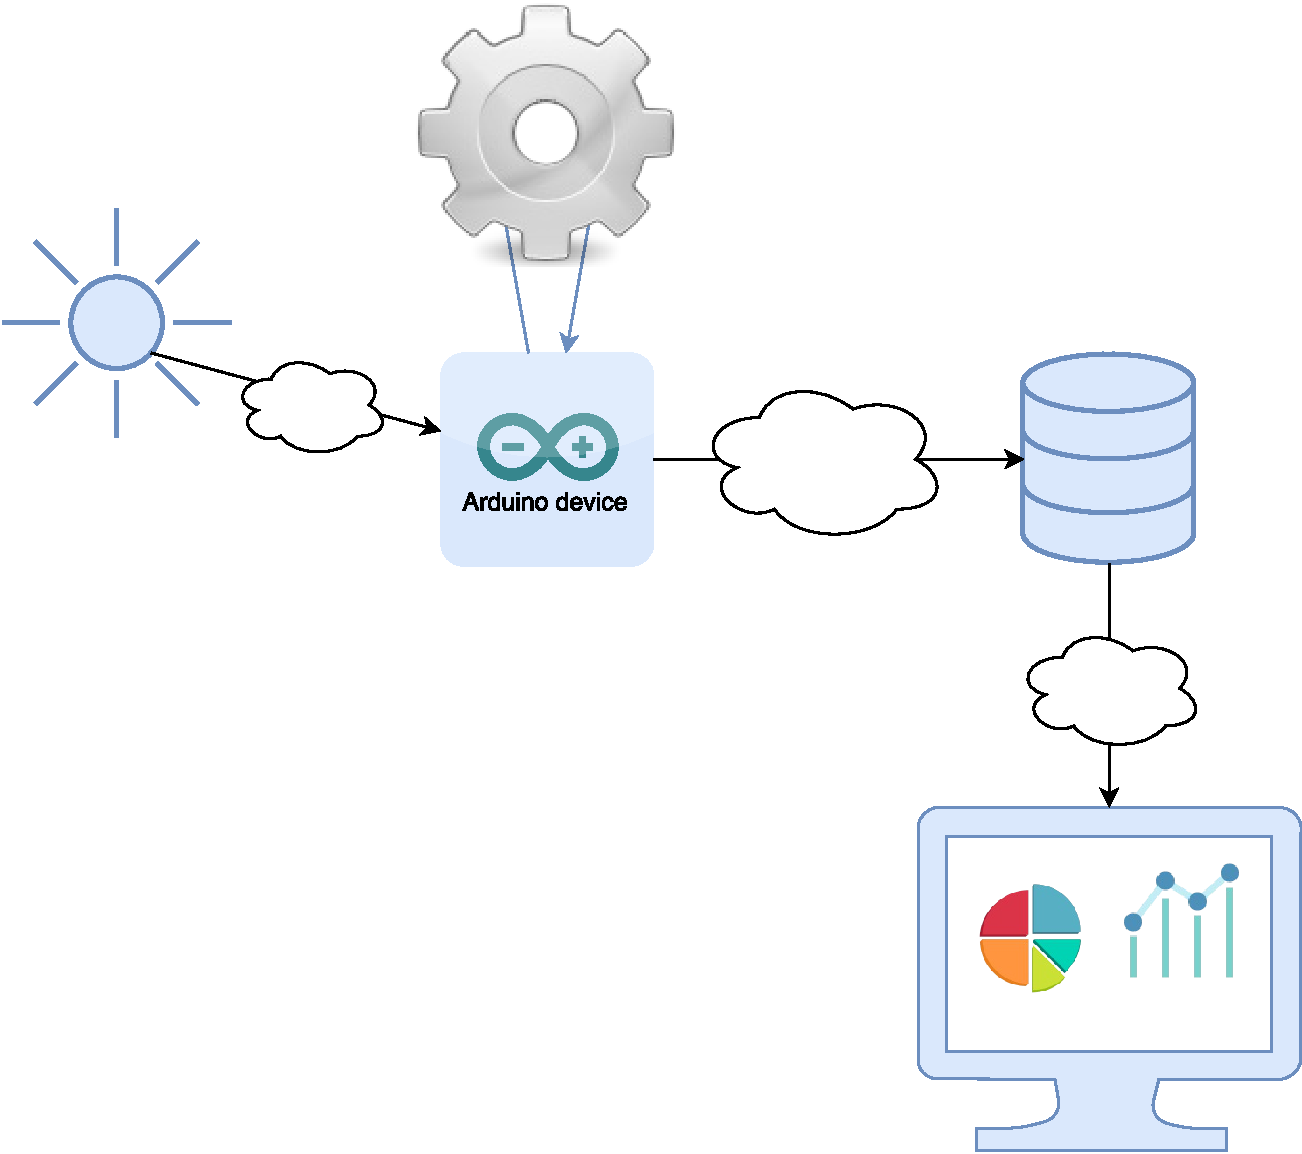
\includegraphics[width=0.5\textwidth]{img/basic_archi}
    }
  \caption[Basic APDL architecture example]{ Visualisation of all the domain
involve in the APDL ecosystem. There are hardware, software, design and
telecommunication. And sometimes, a person doesn’t know any part of this.}
  \label{fig:basic_archi}
\end{figure}

\section{Problem Statement}
\label{sec:intro-problem-statement}

According to the previous example we could say that not everybody could develop
a project like this from scratch. Maybe some people have the whole knowledge to
do this by themselves but not a lambda person.

The big deal is that there is no way to simply create that without involving
multiple people from different domains and bring it together, and that creates
another difficulty: team management, different programming knowledge, the same
understanding of the project, and many more.

\section{Solution Statement}
\label{sec:intro-solution-statement}

The Acquire and Process Description Language \gls{APDL} ecosystem goal is to
provide a simple way to describe such a pipeline. From the sampling of the data
from a sensor and his transformation to the display of the result of charts by
storing them into a database or send them to a specific server.

\section{Roadmap}
\label{sec:intro-roadmap}

TODO

%%% Local Variables:
%%% mode: latex
%%% TeX-master: "../thesis"
%%% End:
